\documentclass[a4paper,12pt]{uninove-ppgi} %courier ou times
\begin{document}
\lstset{
    language=xml,
    tabsize=3,
    frame=shadowbox,
    rulesepcolor=\color{gray},
    xleftmargin=20pt,
    framexleftmargin=15pt,
    keywordstyle=\color{blue}\bf,
    commentstyle=\color{OliveGreen},
    stringstyle=\color{red},
    numbers=left,
    numberstyle=\tiny,
    numbersep=5pt,
    breaklines=true,
    showstringspaces=false,
    basicstyle=\footnotesize,
    emph={food,name,price},emphstyle={\color{magenta}}
}

% Posiciona o logo da Uni9 no topo

\includegraphics[height=1.5cm]{uninove-logo}

% parametros de capa e folha de rosto (é necessário configurar todos)
\Universidade{UNIVERSIDADE NOVE DE JULHO - UNINOVE}

\Autor{EXCLUÍDOS OS DADOS SOBRE OS AUTORES EM ATENDIMENTO A LGPD - LEI GERAL DE PROTEÇÃO DE DADOS}

% ATENÇÃO: NÃO INCLUIR NOME E RA DE NENHUM ALUNO
% EM NENHUMA PARTE DO DOCUMENTO

\Titulo{DROP FLASH}

% Inserir o nome do projeto no formato que está abaixo (Olhe o nome da disciplina na central do aluno)
\Tipoprojeto{PROJETO EM GESTÃO DE SISTEMAS COMPUTACIONAIS}

% Informe qual o curso: Bacharel ou Tecnólogo + curso
\Curso{Ciência da Computação}

% NÃO ALTERAR
\Orientador{Edson Melo de Souza, Dr.}

% Inserir o ano correspondente
\Ano{2024}

% gera a capa automaticamente
\capa

% gera folha de rosto automaticamente
\folharosto

% ##################### Início dos elementos pré-textuais ############################

% Resumo (Obrigatório)
% !TEX root = ..\main.tex

\PalavrasChave{Delivery, Eficiência, Robôs, Drones, Motos, Sustentabilidade.}
\centeredchapterstyle
\begin{resumo}
    \noindent\textbf{}A crescente demanda por serviços de delivery, especialmente em áreas urbanas densamente povoadas, tem gerado preocupações significativas em relação à eficiência e rapidez das entregas. Este estudo propõe soluções para mitigar os desafios associados a essa alta demanda, visando reduzir os tempos de espera e melhorar a experiência do cliente. O objetivo principal desta pesquisa é avaliar a eficácia de diferentes modalidades de entrega, incluindo o uso de robôs, drones e motos elétricas, na otimização da produtividade e na redução dos custos operacionais e ambientais. Para alcançar esses objetivos, foram realizadas investigações tanto individualmente quanto em grupo, além de múltiplas reuniões para discutir os temas pertinentes. Métodos de análise de dados qualitativos e quantitativos foram empregados para avaliar a viabilidade e eficácia das diferentes abordagens de entrega. Os resultados indicam que a implementação de métodos de entrega utilizando robôs, drones e motos elétricas é altamente viável, essas abordagens demonstraram capacidade para aumentar a eficiência das entregas, reduzir os custos operacionais e minimizar o impacto ambiental associado ao transporte de mercadorias. A adoção de tecnologias inovadoras, como robôs, drones e motos elétricas, pode representar uma solução eficaz para os desafios enfrentados no setor de delivery. Além de aumentar a satisfação do cliente através da redução dos tempos de espera, essas soluções também oferecem benefícios significativos para as empresas, incluindo a redução de custos e o aumento do retorno líquido. No entanto, são necessários estudos adicionais para avaliar a implementação prática e a aceitação do mercado dessas tecnologias em larga escala.
\end{resumo}

% Abstract (Obrigatório) - resumo em inglês
% !TEX root = ..\main.tex

\KeyWords{Delivery, Efficiency, Robots, Drones, Motorcycles, Sustainability.}
\centeredchapterstyle
\begin{abstract}
    \noindent\textbf{}The growing demand for delivery services, especially in densely populated urban areas, has raised significant concerns regarding the efficiency and speed of deliveries. This study proposes solutions to mitigate the challenges associated with this high demand, aiming to reduce waiting times and improve the customer experience. The main objective of this research is to evaluate the effectiveness of different delivery modalities, including the use of robots, drones, and electric motorcycles, in optimizing productivity and reducing operational and environmental costs.  To achieve these objectives, investigations were conducted both individually and in groups, along with multiple meetings to discuss pertinent topics. Qualitative and quantitative data analysis methods were employed to assess the feasibility and effectiveness of different delivery approaches. The results indicate that the implementation of delivery methods using robots, drones, and electric motorcycles is highly feasible. These approaches have demonstrated the ability to increase delivery efficiency, reduce operational costs, and minimize the environmental impact associated with the transportation of goods.  The adoption of innovative technologies, such as robots, drones, and electric motorcycles, can represent an effective solution to the challenges faced in the delivery sector. In addition to increasing customer satisfaction by reducing waiting times, these solutions also offer significant benefits for companies, including cost reduction and increased net returns. However, further studies are necessary to evaluate the practical implementation and market acceptance of these technologies on a large scale.
\end{abstract}


% Sumário (Obrigatório)
\begingroup
\makeatletter \let\ps@plain\ps@empty \makeatother
\tableofcontents % sumário
\endgroup
\thispagestyle{empty}

% Lista de figuras
\renewcommand*\listfigurename{Lista de Ilustrações}
\listoffigures
\thispagestyle{empty}

% ############### Fim dos elementos pré-textuais ######################

\regularchapterstyle

% ############### Início dos Capítulos (Obrigatório ) #################
%Introdução
%Base Teórica
%Descrição drones
%Descrição - motos e Bikes
%Descrição rotas
%Financeiro drones e Motos
%Marketing drones e Motos
%Legislação
%Funcionando do site 
%Marketing das motos
%Descrição Robo
%Financeiro/ orçamento
%Apresentação PDF/ Marketing
%Propostas contrato
%Regulamentação
%Conclusão

% Introdução
\chapter{Introdução}
\label{ch:introducao}

     Nasce a Drop Flash quando percebemos que no momento atual do mundo a conveniência e a rapidez são essenciais, é uma empresa de delivery inovadora que busca revolucionar o mercado com seu sistema de entrega eficiente e tecnologicamente avançado. Tudo começou com um grupo de nove empreendedores apaixonados por tecnologia e pela ideia de facilitar a vida das pessoas. Cada membro da equipe trouxe consigo habilidades únicas e experiências diversas, formando um time poderoso e determinado a fazer a diferença. A história da Drop Flash é marcada pela determinação e pelo espírito empreendedor de seus fundadores. Os motoboys da Drop Flash são parte fundamental dessa operação. Eles utilizam suas próprias motos, conhecendo as ruas da cidade como ninguém, garantindo que as entregas sejam feitas de forma ágil e eficiente. Além disso, a empresa inovou ao introduzir o uso de drones para entregas na região central da cidade, oferecendo uma opção rápida e sustentável para os clientes que precisam de suas encomendas com urgência. Com um sistema de taxas transparente e justo, a Drop Flash quer conquistar a confiança dos clientes e estabelecer parcerias sólidas com diversos estabelecimentos comerciais. \\

     \section{Qual o principal objetivo?}
Temos como objetivo a satisfação do cliente e manter a boa reputação do estabelecimento que utiliza o delivery, e com isso nossa empresa presta esse suporte, trabalhamos com drones e motos que podem ser alugadas por comerciantes que querem uma melhor experiência, rapidez e segurança nas entregas. Baseado em pesquisa feitas com clientes e comerciantes que utilizam do delivery, o problema mais relatado foi sobre o atraso nas entregas. Isso ocorre devido a vários fatores, os principais são tráfego intenso, problemas de logística e falta de profissionais na área, devido a alta demanda os motoboys não dão conta de tantas entregas, e nossos drone vem para inovar o mercado com entregas rápidas e eficientes, eles podem entregar rápido pois evita congestionamentos de trânsito. Os drones também tem uma grande flexibilidade e adaptabilidade, eles podem ser programados para voar em diferentes altitudes e rotas, tornando-os altamente adaptáveis a várias condições climáticas.
     
\section{Sistema de Entregas e Taxas}
 A Drop Flash opera por meio de um sistema que conecta clientes provenientes de diversas plataformas, nas quais o estabelecimento comercial está presente. Dentre essas plataformas, incluem-se serviços de entrega com base de integrações como iFood, WhatsApp, Rappi, delivery direto, entre outros. A Drop Flash assume a responsabilidade pelo sistema de entregas da loja, empregando entregadores independentes para realizar entregas de forma ágil e eficiente. Um dos principais diferenciais reside no uso de drones, reconhecidos pela sua capacidade de realizar entregas com alta precisão e alcançando um padrão de qualidade elevado para o cliente final.

Quanto às taxas de entrega, estas são calculadas levando em consideração a distância percorrida e a demanda da região.

\section{Missão e valores}

Missão: "Facilitar a vida das pessoas, oferecendo soluções de entrega rápidas, seguras e eficientes, utilizando tecnologia de ponta e uma equipe comprometida com a excelência."\\

Valores:
 \begin{itemize}
     \item Eficiência: Priorizamos a entrega rápida e no prazo, utilizando drones e motoboys altamente treinados.
     \item Inovação: Estamos sempre buscando novas tecnologias e formas de aprimorar nossos serviços.
     \item Segurança: Garantimos a segurança tanto dos nossos colaboradores quanto das entregas, seguindo rigorosos padrões de segurança.
     \item Comprometimento: Nosso time é comprometido com a satisfação do cliente e com a qualidade do serviço prestado.
     \item Sustentabilidade: Contribuímos para um mundo mais sustentável ao utilizar tecnologias eco-friendly em nossas operações.
     \item Transparência: Mantemos uma comunicação aberta e transparente com nossos clientes, parceiros e colaboradores.
     \item Respeito: Valorizamos a diversidade e respeitamos as diferenças individuais em nossa equipe e na comunidade onde atuamos.
 \end{itemize}

% Base Teórica
\chapter{Fundamentação Teórica}
\label{ch:identificador}

Baseado no artigo \cite{yanique2023drone} que realiza uma analise SWOT que é uma ferramenta usada para avaliar os pontos fortes, fracos, oportunidades e ameaças de um determinado negócio ou tecnologia.
\begin{itemize}
    \item \textbf{Pontos fortes:} Acessibilidade melhorada – os drones podem fazer entregas em áreas remotas e de difícil acesso, proporcionando melhor acessibilidade para clientes e empresas.
    \item \textbf{Fraquezas:} Capacidade de carga útil limitada – os drones têm capacidade de carga útil limitada, o que significa que podem não ser adequados para pacotes maiores e mais pesados.
    \item \textbf{Oportunidade:} Aumento da demanda – com o tempo houve uma demanda muito grande por métodos de entrega mais rápidos e eficientes, e com isso a entrega feita por drones é uma solução muito atraente.
    \item \textbf{Ameaças:} Percepção publica – a percepção publica sobre os drones pode ser uma ameaça potencial para a indústria, em especifico se os drones forem visto como um incomodo ou ameaça a segurança pública.
\end{itemize}

    \section{Vantagens, economia e desafios}

Vantagens e Potencial Econômico
\begin{itemize}
    \item O uso de drones para entrega de pacotes oferece várias vantagens em relação aos métodos tradicionais. Eles proporcionam maior flexibilidade, acessibilidade e eficiência na entrega, além de benefícios ambientais, como a redução de emissões de CO2 quando comparados a veículos movidos a gasolina \cite{cornell2023drones}.
    \item As vantagens econômicas e ambientais sugerem que a entrega por drones pode se tornar uma parte importante do ecossistema de entregas. Empresas com visão de futuro planejarão hoje um futuro habilitado para drone \cite{cornell2023drones}.
\end{itemize}

    \section{Desafios tecnológicos e regulatórios}
    
Embora promissores, os drones enfrentam vários desafios. Os custos
operacionais atuais são altos, principalmente devido à necessidade de operadores humanos monitorando cada drone. Para que os drones se
tornem mais competitivos, será necessário avançar em tecnologias de voo autônomo e na gestão de tráfego aéreo, permitindo que um operador gerencie vários drones simultaneamente \cite{cornell2023drones}. Além disso, as regulamentações precisam evoluir para permitir uma maior densidade de drones no espaço aéreo urbano.

    \section{Melhora nas entregas}

No artigo \cite{Submit2022} faz a citação que os drones podem realizar entregas de forma significativamente mais rápida do que os métodos tradicionais. Foi realizado um teste em Belo Horizonte (MG), o tempo de delivery caiu de 40 minutos para 5 minutos.

	\section{Steve Robot Express}

Com Base em pesquisas, procuramos trabalhar com o objetivo de pesquisa em informações advinda de autores que pudessem fundamentar uma base de reflexões teóricas e práticas para contribuir na criação da nossa empresa focando nas novas modalidades de entregas autônomas e mais sustentáveis por robôs Autônomos.

De acordo com \cite{Bakach2020} a utilização de robôs poderia contribuir para a redução dos custos como das emissões de gases do efeito estuda (GEE) e redução de congestionamento em grandes cidades. Também devemos pensar nos desafios de se viabilizar todo esse processo de utilização dos robôs autônomos abordando os desafios de agendar entregas utilizando os robôs \cite{BoysenN2018}. Podemos nos basear em cálculos matemáticos que nos fornecem dados valiosos para o aprimoramento dos robôs a cada entrega realizada. 

Outra possibilidade seria em áreas de pilotagem de aeronaves por exemplos próximos de campos de voos e aeroportos \cite{faa2018} onde os robôs enfrentam menos regulamentações de segurança do que a de drones.

Empresas como Starship Technologies, Robby, Amazon Scout e Synkar já estão vendendo ou desenvolvendo robôs de entrega buscando ganhar espaço em um mercado de robôs de serviço que prevê um aumento na demanda de entregas nos próximos anos com o envelhecimento da população e aumento na demanda por entregas. (Boston Consulting Group (BCG)) (Mordor Intelligence Research \& Advisory).


% Modelos de drones utilizados
\chapter{Drones}
\label{ch:identificador}

\section{DLV-1}

Possui uma capacidade de 2.5 kg de carga, podendo decolar com até 12.5 kg podendo percorrer 3km de ida e volta.

\begin{figure}[!ht]
    \centering
    \caption{Drone DLV-1 Drop Flash.}
    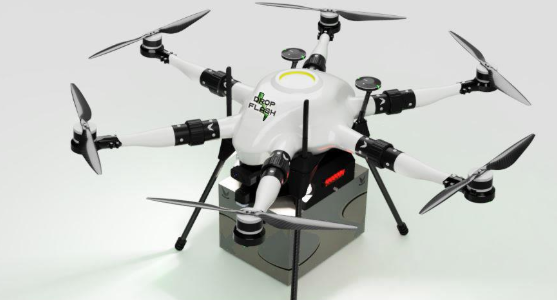
\includegraphics[width=0.6\textwidth]{figuras/DLV1.png}
    \label{fig:DLV1}\\
    \small Fonte: \url{https://www.speedbird.aero}
\end{figure}

O DLV-1 é interessante para entregas mais rápidas e leves, como documentos e artigos de farmácia, que necessitam de um tempo menor de entrega por conta de sua possível urgência\cite{Speed2024}.

\section{DLV-2}

Possui uma capacidade de 6 kg de carga e pode decolar com 25 kg de carga com 8km de ida e volta.

\begin{figure}[!ht]
    \centering
    \caption{Drone DLV-2 Drop Flash.}
    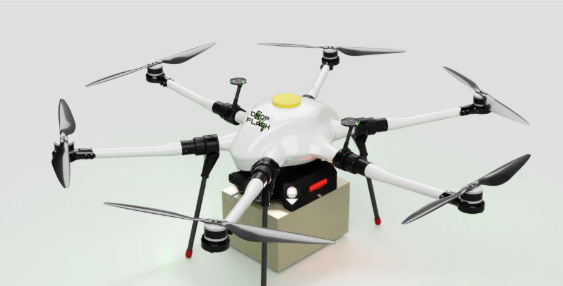
\includegraphics[width=0.6\textwidth]{figuras/Dlv 2.png}
    \label{fig:DLV2}\\
    \small Fonte: \url{https://www.speedbird.aero}
\end{figure}

O DLV-2 será utilizado para entregas de maior peso, interessante para compras no mercado ou um pedido para mais pessoas em um restaurante\cite{Speed2024}.

\section{DLV-4}

Possui uma capacidade de carga de até 5 kg, com peso máximo de decolagem dem25 kg, porém o diferencial do DLV-4 é a distância que pode percorrer, que é de até 40km de ida e volta.

\begin{figure}[!ht]
    \centering
    \caption{Drone DLV-4 Drop Flash.}
    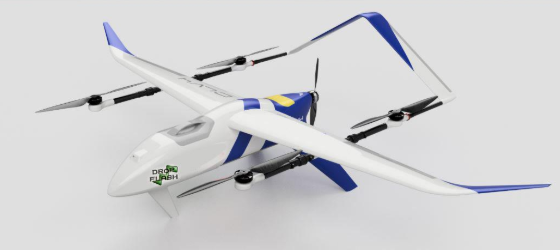
\includegraphics[width=0.6\textwidth]{figuras/dlv 4.png}
    \label{fig:DLV2}\\
    \small Fonte: \url{https://www.speedbird.aero}
\end{figure}


O DLV-4 entrega uma proposta diferente dos demais, pois tem a capacidade de realizar viagens mais longas, portanto se um cliente mora no interior ou afastado de um estabelecimento de seu interesse, é possível realizar pedidos de cidades e bairros vizinhos\cite{Speed2024}.

\section{Tecnologia utilizada nas entregas}

Os drones terão uma tecnologia que iça e baixa as cargas por meio de um cabo de aço, agilizando o procedimento de entrega. Dessa forma não existe a necessidade do drone descer até o solo para realizar a entrega, assim facilitando e a mantendo mais seguro esse procedimento\cite{Wing2024}.

\begin{figure}[!ht]
    \centering
    \caption{Exemplo de uma entrega através do cabo de aço..}
    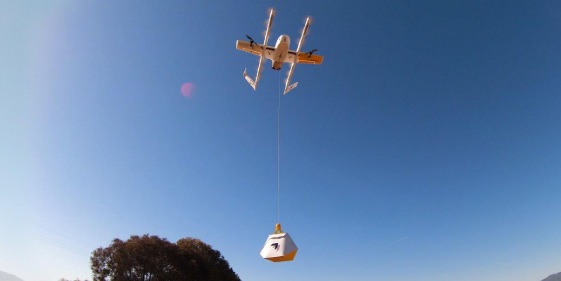
\includegraphics[width=0.6\linewidth]{figuras/tec utlzd.png}
    \label{fig:DLV2}\\
    \small Fonte: \url{https://wing.com/how-it-works/}
\end{figure}



O cabo de aço utilizado será de 3,18 mm de diâmetro com comprimento de 30 metros, que soma em 900 gramas o peso de carga do drone. O cabo em questão é forte o suficiente para suportar o peso e fino o suficiente para não sobrecarregar a carga.

\section{Pontos de decolagem e pouso}

Para cada região cadastrada existirá uma base para pouso, decolagem e manutenção dos drones. No total serão 9 bases e cada base terá 20 DLV-1, 20 DLV-2 e 10 DLV-4\cite{Speed2024}.

\begin{figure} [!ht]
    \centering
    \caption{Ilustração de um ponto de pouso e decolagem de drones da Drop Flash.}
    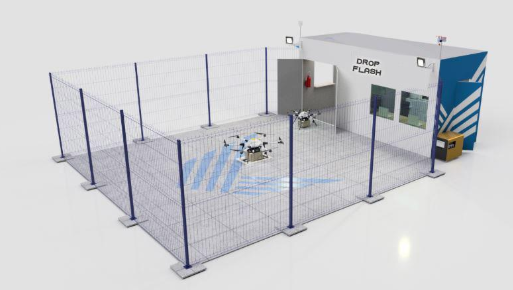
\includegraphics[width=0.6\linewidth]{figuras/p dec e po.png}
    \label{fig:enter-label}\\
    \small Fonte: \url{https://www.speedbird.aero}
\end{figure}

% Motos e bikes
\chapter{Motos}
\label{ch:identificador}
	\section{Motos Elétricas}
 
 Além da disponibilidade de drones os nosso serviços fornecem as motos elétricas que são divididas em 3 classes \textbf{(OLA S1 Pro, OLA S1 Air e OLA S1X)} ,nos quais as motos são uma opção quando os serviços de drones não estiverem disponíveis, por conta de qualquer fator.\\
 
A moto \textbf{S1 Pro} tem um alcance de 195 km tendo uma performance de 120km/por hora, sendo a mais veloz que será atribuída para as entregas mais urgentes.\\

\begin{figure} [!ht]
    {\centering
    \caption{S1 Pro roxa}
    \includegraphics[height=0.3\linewidth]{figuras/S1 Pro.png}
    \label{fig:enter-label}
    \fonte{Ola Electric}
    }
\end{figure}

A moto \textbf{S1 Air} possui um alcance de 151 km com uma taxa de 90 km/ por hora podendo ser utilizada em bairros medianos não muito grandes.\\

\begin{figure} [!ht]
   { \centering
    \caption{S1 Air verde}
    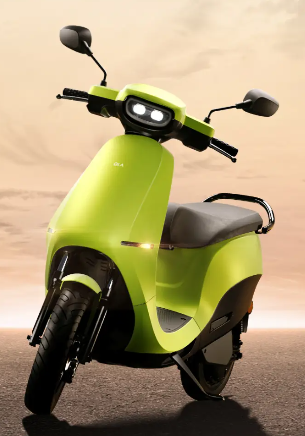
\includegraphics[height=0.3\linewidth]{figuras/S1 AIR.png}
    \label{fig:enter-label}
    \fonte{Ola Electric}
    }
\end{figure}

Já a \textbf{S1X} tem um alcance de 190 km com uma velocidade de 90km/por hora que possivelmente será a moto mais utilizada no dia a dia por conta da sua distância de alcance com carga máxima e de sua velocidade.

\begin{figure} [!ht]
    {\centering
    \caption{S1X vermelho}
    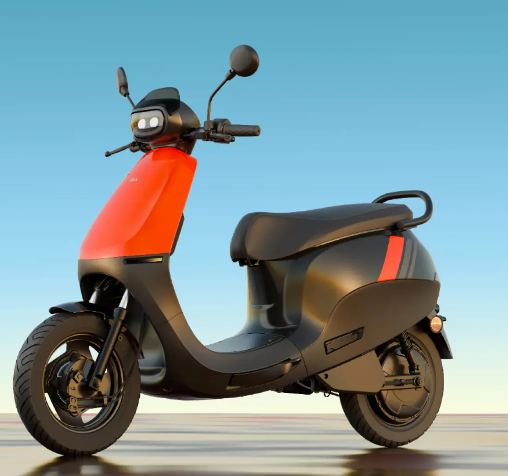
\includegraphics[height=0.2\linewidth]{figuras/S1X.png}
    \label{fig:enter-label}
    \fonte{Ola Electric}
    }
\end{figure}

   \section{Motos Convencionais}

   A nossa empresa tem um foco em preservar o meio ambiente por isso focamos em meios de transportes elétricos porém os nossos motoboys terão a opção de utilizar as motos movidas a gasolina por conta de qualquer fator por exemplo: se sentir mais à vontade ou por ter mais experiências com as motos a gasolina.\\ 
   
   Para motos a gasolina teremos como fabricantes a empresa Honda com os seguintes modelos:
   
   Honda Drop 110i pode ter uma performance de alcance de 200 km com uma média de 40 a 50 km/por hora.\\

   \begin{figure} [!ht]
       {\centering
       \caption{Moto Drop - 110i}
       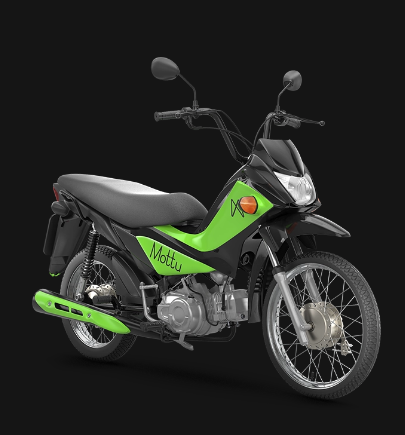
\includegraphics[height=0.3\linewidth]{figuras/Drop110.png}
       \label{fig:enter-label}
       \fonte{https://mottu.com.br/aluguel/}
       }
   \end{figure}
   
   Já a Honda Drop Sport 160 pode alcançar uma faixa de 500 km com a média de distância sendo de 40 km. 

   \begin{figure} [!ht]
       {\centering
       \caption{Moto Drop Sport 160}
       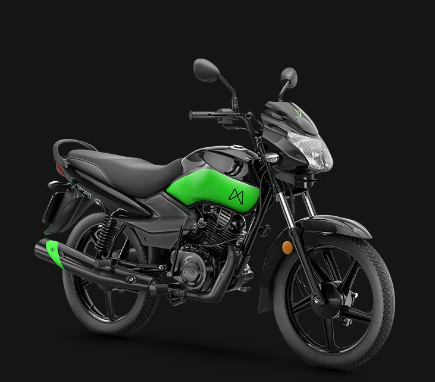
\includegraphics[height=0.2\linewidth]{figuras/Drop Sport160.png}
       \label{fig:enter-label}
       \fonte{https://mottu.com.br/aluguel/}
       }
   \end{figure}

% Rotas dos drones
\chapter{Rotas dos drones}
\label{ch:identificador}
  
O uso de drones da nossa empresa tem como objetivo tornar as entregas mais rápidas no menor tempo possível e ter um aumento nos números de entregas com uma estimativa da média de 336 mil entregas por bairro sendo utilizado no total em nove bairros mas incrementamos em dois bairros como um exemplo de como seria.\\
Os drones em si teriam uma tecnologia de cálculo de rotas com uma análise rápida para obter uma certa agilidade, cada ponto de apoio teria uma equipe totalmente treinada com esse tipo de serviço além de certificados comprovando que são capazes do manuseio de drones com total eficiência.\\
Uma das maneiras que poderiam ser solicitadas às entregas seria da seguinte forma: os nossos serviços seriam solicitados, o drone iria levar a encomenda até a base para completar a entrega e o entregador ‘’motoboy’’ iria só a finalizar.

 \section{Bela Vista}

Bela Vista é um bairro relativamente pequeno quando o assunto é acrescentar drones para entrega, tendo um raio aproximadamente 2,6 km² com uma população de cerca de 70 mil habitantes. Esse bairro por si só tem uma certa fama pois é conhecido como o bairro do Bixiga, sendo uma das suas lendárias atrações paulistas além de teatros e do Museu de Arte de São Paulo.\\
Na imagem abaixo mostra que nesse bairro que não é muito grande, nos instalaremos uma única base de apoio tendo nela 10 drones disponíveis, monitorados por uma equipe especializada com certificado para o uso de drones com um regulamento de manter uma certa distância das pessoas pelo menos 30 metros e com a altura do voo do drone de 50 metros seguindo as mesmas rotas das nossas motos porém com mais rapidez. 

\begin{figure} [!ht]
   { \centering
   \caption{Rota do drone no bairro Bela Vista}
    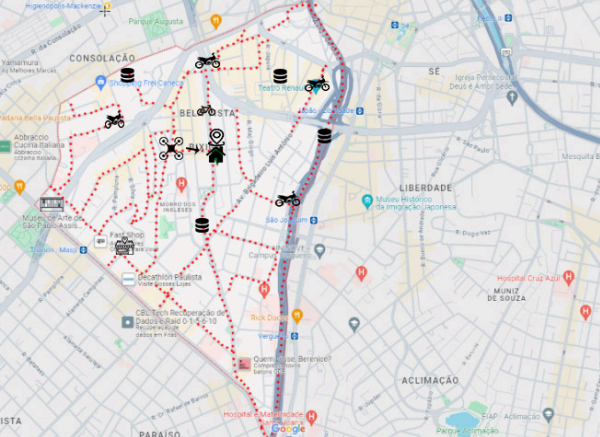
\includegraphics[width=0.5\linewidth]{figuras/rota bela vista.png}
    \label{fig:enter-label}
    \fonte{https://maps.app.goo.gl/8MuL8D5QTETv6svq8}
    }
\end{figure}

 \section{Santa Cecília}

 O Bairro de Santa Cecília, localizado na zona central do município de São Paulo, abrange uma área de aproximadamente 2,1 km². É um espaço onde o tradicional e o moderno convivem em harmonia, oferecendo uma rica experiência cultural e culinária aos seus moradores e visitantes, tendo uma população aproximadamente
de 15 mil habitantes. Santa Cecília possui alguns pontos turísticos como: Paróquia de Santa Cecília, Praça Frederico Arbegaus, Estátua do Gaúcho entre outras, além de sua própria história, contendo várias crises e mudanças e contendo seu renascimento
como um novo bairro.\\
Logo abaixo temos uma imagem de como seria a implementação dos drones nesse bairro escolhido, seguindo todas as normas e regulamentações para o uso de drones.

\begin{figure} [!ht]
    {\centering
    \caption{Rota do drone no bairro Santa Cecília}
    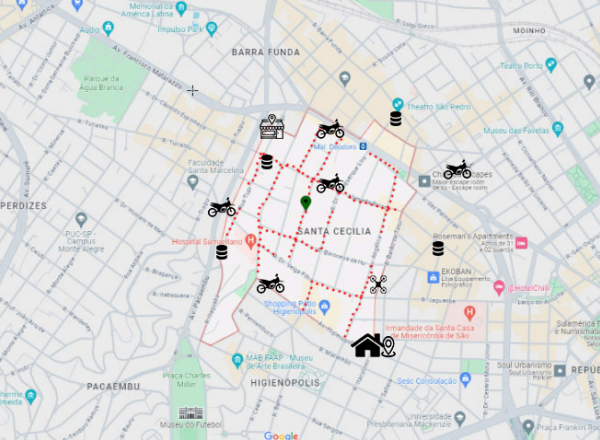
\includegraphics[width=0.9\linewidth]{figuras/rota santa cecilia.png}
    \label{fig:enter-label}
    \fonte{https://maps.app.goo.gl/YwaVA79U32ioDPiz8}
    }
\end{figure}



% Fianceiro moto e drone
\chapter{Financeiro dos meios de transporte}
\label{ch:identificador}
\section{Bairros e Faturamento}

\textbf{Bela Vista}
\begin{itemize}
    \item Raio: 2,6 km
    \item Comércios: 11.970
    \item Média: R\$ 143,64/ R\$ 12,00 / 2,6 km
    \item Semanal: R\$ 143,64 *7 = R\$ 1.005,48
    \item Mensal: R\$ 143,64 *30 = R\$ 4.309,2
\end{itemize} \\

\textbf{Bom Retiro}
\begin{itemize}
    \item Raio: 1.055 km
    \item Comércios: 10.036
    \item Média: R\$ 138,99/ R\$ 14,61/1,055 km
    \item Semanal: R\$ 138,99*7 = R\$ 972,93
    \item Mensal: R\$ 138,99*30 = R\$ 4.169,7
\end{itemize}\\

\textbf{Cambuci}
\begin{itemize}
    \item Raio: 3,9 km
    \item Comércios: 9.758
    \item Média: R\$ 258,58/ R\$ 26,50 / 3,9 km
    \item Semanal: R\$ 258,58*7 = R\$ 1.810,06
    \item Mensal: R\$ 258,58*30 = R\$ 7.757,4
\end{itemize}\\

\textbf{Consolação}
\begin{itemize}
    \item Raio: 85,9 km
    \item Comércios: 13.703
    \item Média: R\$ 16,210,64/1183,00 / 85,9 km
    \item Semanal: R\$ 16,210,64*7 = R\$ 113.474,48
    \item Mensal: R\$ 16,210,64*30 = R\$ 486.319,2
\end{itemize}\\ 

\textbf{Higienópolis}
\begin{itemize}
    \item Raio: 3,5 km
    \item Comércios: 7.979 Pontos:
    \item Média: R\$ 315,17/39,50 / 3,5 km ≈ R\$ 11,29 por km.
    \item Semanal: R\$ 315,17*7 = R\$ 2.206,19
    \item Mensal: R\$ 315,17*30 = R\$ 9.455,1
\end{itemize}\\

\textbf{Liberdade}
\begin{itemize}
    \item Raio: 3,7 km
    \item Comércios: 9.422
    \item Média: R\$ 396,66/42,10 / 3,7 km ≈ R\$ 11,378 por km
    \item Semanal: R\$ 396,66*7 = R\$ 2.776,62
    \item Mensal: R\$ 396,66*30 = R\$ 11.899,8
\end{itemize}\\

\textbf{República}
\begin{itemize}
    \item Raio: 2,3 km
    \item Comércios: 9.937
    \item Média: R\$ 244,45/R24,60 / 2,3 km ≈ R\$ 10,70 por km.
    \item Semanal: R\$ 244,45*7 = R\$ 1.711,15
    \item Mensal: R\$ 244,45*30 = R\$ 7.333,5
\end{itemize}\\

\textbf{Santa Cecília}
\begin{itemize}
    \item Raio: 2,1 km
    \item Comércios: 9.351
    \item Média: R\$ 93,51/10,00 / 2,1 km ≈ R\$ 4,76 por km.
    \item Semanal: R\$ 93,51 * 7 = R\$ 654,57
    \item Mensal: R\$ 93,51 * 30 = R\$ 2.805,3
\end{itemize}\\

\textbf{Sé}
\begin{itemize}
    \item Raio: 2,1 km
    \item Comércios: 4.473
    \item Média: R\$ 44,73/10,00 / 2,1 km ≈ R\$ 4,76/km.
    \item Semanal: R\$ 44,73 * 7 = R\$ 313,11
    \item Mensal = R\$ 44,73 * 30 = R\$ 1.341,90
\end{itemize}


\section{Despesas}

Meios de Transportes: será usado modelos de motociatas elétricas da montara indiana OLA e drones para entregas da empresa SPEEDBIRD além dos funcionários de todos os ramos atuando na companhia.

\section{Motocicleta Elétrica}

\begin{figure} [!ht]
    {\centering
    \caption{S1 Pro roxa}
    \includegraphics[height=0.3\linewidth]{figuras/S1 Pro.png}
    \label{fig:enter-label}
    \fonte{Ola Electric}
    }
\end{figure}

Aluguel será:
\begin{itemize}
    \item Diário: R\$ 20,00
    \item Semanal: R\$ 40,00
    \item Mensal: R\$ 100,00
\end{itemize}

Especificações: 
\begin{itemize}
    \item Espaço para bagageira - 34L.
    \item Velocidade máxima - 120 km/h.
    \item Alcance certificado de 195 km.
    \item Aceleração - 0 a 40 em 2,6 segundos.
    \item Liberte o poder de um motor de 11kW.
\end{itemize}

\begin{figure} [!ht]
   { \centering
    \caption{S1 Air verde}
    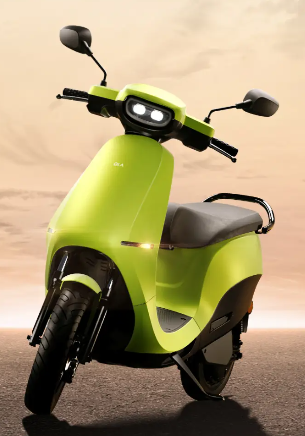
\includegraphics[height=0.3\linewidth]{figuras/S1 AIR.png}
    \label{fig:enter-label}
    \fonte{Ola Electric}
    }
\end{figure}

Aluguel será: 

\begin{itemize}
    \item Diário: R\$ 30,00
    \item Semanal: R\$ 50,00
    \item Mensal: R\$ 150,00
\end{itemize}

Especificações:

\begin{itemize}
    \item 151 KM de alcance.
    \item Espaço para bagageira de 34L
    \item Aceleração - 0-40 em 3,3 seg.
    \item Velocidade máxima de 90 km/h.\\\\\\\\\\\\\\\\\\
\end{itemize}

\begin{figure} [!ht]
    {\centering
    \caption{S1X vermelho}
    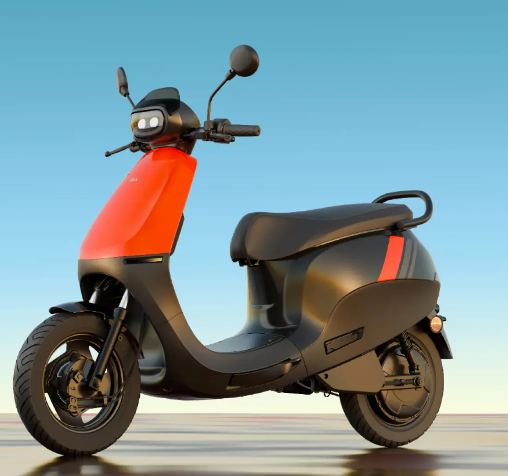
\includegraphics[height=0.2\linewidth]{figuras/S1X.png}
    \label{fig:enter-label}
    \fonte{Ola Electric}
    }
\end{figure}

Aluguel será: 
\begin{itemize}
    \item Diário: R\$ 50,00
    \item Semanal: R\$ 90,00
    \item Mensal: R\$ 350,00
\end{itemize}

Especificações:
\begin{itemize}
    \item 190 KM de alcance.
    \item Espaço para bagageira de 34L
    \item Aceleração: 0-40 em 3,3 seg.
    \item Velocidade máxima: 90 km/h.
\end{itemize}

Aplicativo Ola Electric controle sua scooter direto do seu telefone.

\begin{figure} [!ht]
    {\centering
    \caption{Aplicativo Ola Electric}
    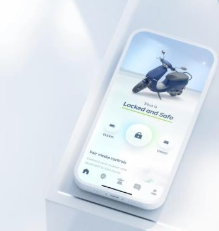
\includegraphics[height=0.4\linewidth]{figuras/app ola.png}
    \label{fig:enter-label}
    \fonte{Ola Electric}
    }
\end{figure}

Um mecânico de motos é de R\$ 1.512,00.
Um Entregador é de R\$ 1.706,00.

\section{Drones}

DLV-1 Possui uma capacidade de 2.5 kg de carga, podendo decolar com até 12.5 kg podendo percorrer 3 km de ida e volta.

\begin{figure}[!ht]
    \centering
    \caption{Drone DLV-1 Drop Flash.}
    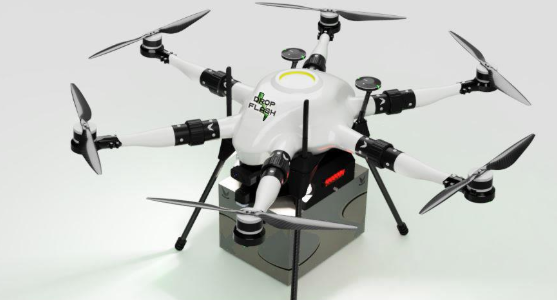
\includegraphics[width=0.6\textwidth]{figuras/DLV1.png}
    \label{fig:DLV1}\\
    \small Fonte: \url{https://www.speedbird.aero}
\end{figure}

Aluguel será: 
\begin{itemize}
    \item Diário: R\$ 100,00
    \item Semanal: R\$ 200,00
    \item Mensal: R\$ 500,00
\end{itemize}

Possui uma capacidade de 6 kg de carga e pode decolar com 25 kg de carga com 8 km de ida e volta.

\begin{figure}[!ht]
    \centering
    \caption{Drone DLV-2 Drop Flash.}
    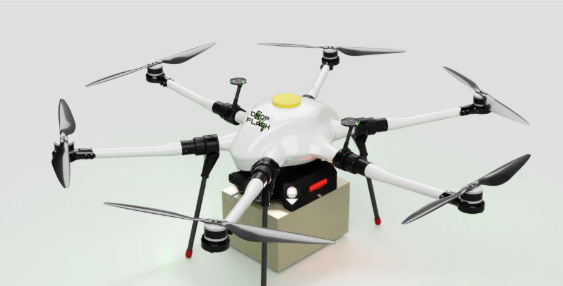
\includegraphics[width=0.6\textwidth]{figuras/Dlv 2.png}
    \label{fig:DLV2}\\
    \small Fonte: \url{https://www.speedbird.aero}
\end{figure}

Aluguel será: 
\begin{itemize}
    \item Diário: R\$ 200,00
    \item Semanal: R\$ 500,00
    \item Mensal: R\$ 1000,00
\end{itemize}

DLV-4 Possui uma capacidade de carga de até 5 kg, com peso máximo de decolagem de 25 kg, porém o diferencial do DLV-4 é a distância que pode percorrer, que é de até 40 km de ida e volta.

\begin{figure} [!ht]
   { \centering
    \caption{Drone DLV-4 Drop Flash.}
    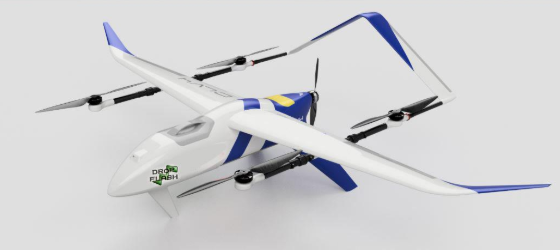
\includegraphics[width=0.6\linewidth]{figuras/dlv 4.png}
    \label{fig:enter-label}
    \fonte{https://www.speedbird.aero}
    }
\end{figure}

Aluguel será: 

\begin{itemize}
    \item Diário: R\$ 500,00
    \item Semanal: R\$ 1000,00
    \item Mensal: R\$ 3000,00
\end{itemize}

\section{Geral}

Pontos de decolagem e pouso Para cada região cadastrada existirá uma base para pouso, decolagem e manutenção dos drones. No total serão 9 bases e cada base terá 20 DLV-1, 20 DLV-2 e 10 DLV-4.

\begin{figure} [!ht]
    \centering
    \caption{Ilustração de um ponto de pouso e decolagem de drones da Drop Flash.}
    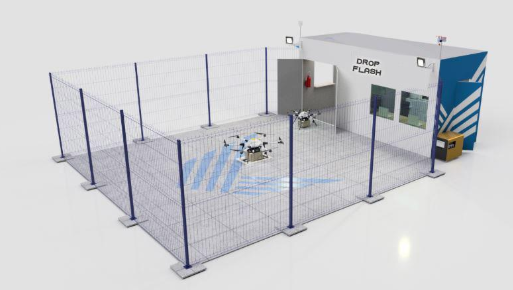
\includegraphics[width=0.4\linewidth]{figuras/p dec e po.png}
    \label{fig:enter-label}
    \fonte{https://www.speedbird.aero}
\end{figure}

Investimento total no drones será de 500 mil. Além doas aluguéis dos terraços dos prédios que media fica em R\$ 5.000,00 mais a parte de instalação e gasto com a rede elétrica variando dependo do lugar. Na parte dos salários um piloto de drone de carga habilitado é em média de R\$ 21.047,00.

\section{Programas}
O Cloud Control Station (CCS) do Speedbird é um poderoso conjunto de software projetado para fornecer infraestrutura tecnológica ponta a ponta para controle e monitoramento de aeronaves, proporcionando uma experiência de usuário segura e contínua. Os operadores podem planejar e definir corredores aéreos e rotas predefinidas para conectar droneportos estrategicamente localizados em cidades, hospitais, armazéns e centros de distribuição.

\begin{figure}[!ht]
  {  \centering
    \caption{Monitoramento das aeronaves}
    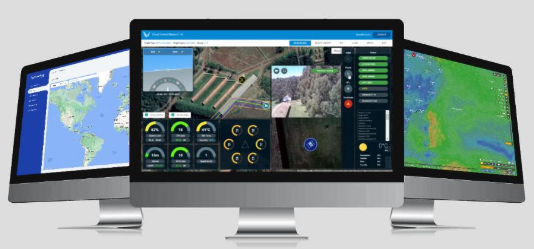
\includegraphics[width=0.5\linewidth]{programa.png}
    \label{fig:enter-label}
    \fonte{https://www.speedbird.aero}
    }
\end{figure}

Na parte dos Softwares de drones e motos será de R\$ 7.000,00 contando peças, internet 4G e 5G e atualizações dos mesmos

% Marketing drone e moto
\chapter{Marketing da empresa}
\label{ch:identificador}

COMO FUNCIONA O MARKETING DA NOSSA EMPRESA

\section{O meio ambiente}
Nossa empresa promove uma ideia que além de pensar em melhorias nas entregas em delivery, pensamos também sobre o nosso meio ambiente, e o uso dos drones pode ajudar em alguns aspectos, observe:\\

\textbf{Redução de emissões de gases de efeito estufa:} As motos movidas a combustível fóssil contribuem para a poluição do ar, emitindo dióxido de carbono e outros poluentes. Os drones elétricos, por outro lado, não emitem gases de escapamento, o que reduz significativamente as emissões de carbono.\\

\textbf{Menor consumo de combustível:} Os drones consomem muito menos energia do que as motos para realizar entregas. Isso significa uma redução no consumo de combustível, que é geralmente derivado de fontes não renováveis, como o petróleo.\\

\textbf{Redução do tráfego nas estradas:} A substituição de motos por drones pode ajudar a diminuir o congestionamento nas estradas, já que os drones podem voar diretamente para o seu destino, evitando o trânsito terrestre. Menos veículos nas estradas também significam menos congestionamento e menos tempo perdido no tráfego.\\

\textbf{Promoção da inovação em energia limpa:} A transição para drones de entrega impulsiona o desenvolvimento e a adoção de tecnologias de energia limpa, como baterias mais eficientes e sistemas de propulsão elétrica. Isso pode ter efeitos positivos em outras áreas, incentivando o uso de energias renováveis e tecnologias mais limpas em diferentes setores\cite{Ifood2022}\cite{Ifood2021}. 

\section{Benefícios de se utilizar drones para entregas}

\textbf{Velocidade e eficiência:} Os drones podem voar diretamente para o seu destino, evitando congestionamentos de trânsito e rotas mais longas. Isso pode resultar em tempos de entrega significativamente mais curtos, especialmente em áreas urbanas.\\

\textbf{Acesso a áreas remotas:} Em regiões com infraestrutura de transporte subdesenvolvida ou em áreas remotas, os drones podem proporcionar uma maneira rápida e eficiente de realizar entregas, alcançando locais que seriam difíceis ou impossíveis de acessar por veículos terrestres.\\

\textbf{Redução de custos:} Embora os custos iniciais de implementação de sistemas de entrega por drones possam ser altos, a operação contínua tende a ser mais econômica do que os métodos tradicionais de entrega, especialmente a longo prazo. Isso inclui economias em combustível, manutenção de veículos e custos de mão de obra.\\

\textbf{Flexibilidade e escalabilidade:} Os drones podem ser facilmente adaptados para uma variedade de cargas e tamanhos de pacotes, desde pequenos itens até mercadorias maiores e mais pesadas. Além disso, a frota de drones pode ser facilmente escalada para atender à demanda sazonal ou flutuações de pedidos.\\

\textbf{Redução de emissões e impacto ambiental:} Como mencionado anteriormente, os drones elétricos não emitem poluentes atmosféricos durante o voo, o que contribui para a redução das emissões de gases de efeito estufa e a melhoria da qualidade do ar, comparado aos veículos terrestres movidos a combustíveis fósseis\cite{Ifood2022}\cite{Ifood2021}.

\section{Tráfego Pago}

Nossa empresa utiliza o método do tráfego pago para divulgação virtual do nosso produto. O tráfego pago nada mais é do que investir em plataformas de anúncios para divulgar seu site ou produto, fazendo assim com que seu produto seja mostrado mais frequentemente ao público, resultando em mais visibilidade e vendas.\\

Quais as vantagens do tráfego pago?\\

\textbf{Resultados imediatos:} Uma das maiores vantagens do tráfego pago é a capacidade de gerar resultados quase imediatos. Assim que uma campanha de publicidade é configurada e ativada, os anúncios podem começar a ser exibidos para o público-alvo, o que pode resultar em um aumento rápido no tráfego para o site ou oferta.\\

\textbf{Foco nas conversões:} o foco do tráfego pago é principalmente as conversões, empresas que pagam pelos anúncios, esperam que elas tenham um retorno significativo em vendas. As plataformas de publicidade online oferecem opções avançadas de segmentação que permitem direcionar os anúncios para públicos específicos com base em uma variedade de critérios, como idade, gênero, interesses, comportamento online, localização geográfica e muito mais. Isso ajuda a garantir que os anúncios sejam exibidos para as pessoas certas, aumentando a relevância e a eficácia da campanha.\\

\textbf{Flexibilidade de orçamento:} O tráfego pago oferece flexibilidade em termos de orçamento, permitindo que empresas de todos os tamanhos e setores participem. Os anunciantes podem definir um orçamento diário ou total para suas campanhas e ajustá-lo conforme necessário com base no desempenho e nos resultados obtidos.\\

\textbf{A estratégia direcionada por dados:} Pelo tráfego pago, é possível reunir informações sobre como os anúncios estão performando e quem é o público-alvo. Esse conhecimento possibilita aprimorar a estratégia continuamente, visando melhorar os resultados ao longo do tempo. Com base nessas análises, é viável adaptar a estratégia para aumentar o número de cliques, conversões e vendas\cite{Semrush2023}.

\section{Nossos drones}

Nós trabalhamos com três tipos de drones na nossa empresa, sendo eles:

\begin{figure} [!ht]
   {\centering
    \caption{DFH - 1}
    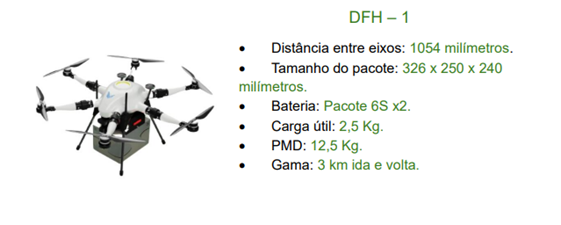
\includegraphics[width=0.9\linewidth]{figuras/drone dfh1.png}
    \label{fig:enter-label}
    \fonte{https://www.speedbird.aero/}
    }
\end{figure}

\begin{figure} [!ht]
    {\centering
    \caption{DFH - 2}
    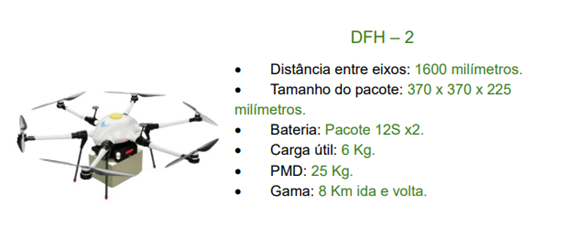
\includegraphics[width=0.9\linewidth]{figuras/drone dfh2.png}
    \label{fig:enter-label}
    \fonte{https://www.speedbird.aero/}
    }
\end{figure}

\begin{figure} [!ht]
 {   \centering
    \caption{DFH - 4}
    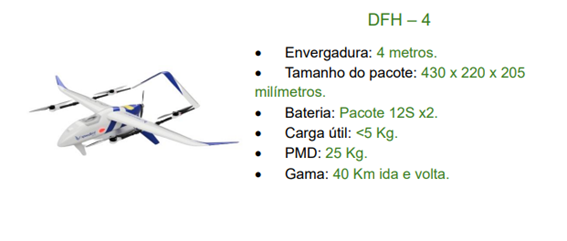
\includegraphics[width=0.9\linewidth]{figuras/drone dfh4.png}
    \label{fig:enter-label}
    \fonte{https://www.speedbird.aero/}
    }
\end{figure}



% Legislação
\chapter{Legislação}
\label{ch:identificador}

\section{Normas para o uso de drone no Brasil}

Segundo a Norma ICA 100 - 40 \cite{(ICA100)} e a RBAC-E Nº 94 EMENDA Nº 03 \cite{(RBAC-E)} para os drones da empresa Drop Flash operarem é necessário seguir a risca as seguintes regras de voo:\\

RPA de peso máximo de decolagem superior a 250g e até 25kg (classe 3) - Em VLOS de 40m até 120m acima do nível do solo. 

\begin{enumerate}
    \item Ter idade igual ou superior a 18 anos para pilotar;
    \item Serão obrigatórias licença e habilitação emitidas pela ANAC (Agência Nacional de Aviação Civil);
    \item Registro emitido junto à ANAC e sua identificação na aeronave; (Obteremos uma aeronave já cadastrada na ANAC).
    \item Apólice de seguro ou certificado de seguro com comprovante de pagamento com cobertura de danos a terceiros (seguro reta);
    \item Documento que contém a avaliação de risco operacional elaborada pelo operador conforme E-94-003 da ANAC; (E-94-003 tem o modelo, instruções e exemplos de como fazer a avaliação de risco operacional).
    \item Manual completo do drone;
    \item Certificado de homologação na ANATEL (Agência Nacional de Telecomunicações) ou número de homologação na ANATEL gravado na aeronave;(obteremos um drone já homologado).
    \item Autorização de voo emitida pelo DECEA (Departamento de Controle do Espaço Aéreo); (Solicitação de voo pelo sistema SARPAS, tempo para aprovação é de 45 minutos, para solicitar voo é necessário o registro emitido pela ANAC e a homologação na ANATEL. Serviço gratuito).
    \item Conhecer os meios de contato do órgão regional responsável pela área de operação;
    \item Conhecer os meios de contato com o órgão ATS mais próximo da área de operação; (Órgão ATS “órgão dos serviços de tráfegos”, ou seja, DECEA e seus subordinados).
    \item Operar em condições VMC; (Condições meteorológicas, expressas em termos de visibilidade, distância de nuvens e teto, iguais ou superiores aos mínimos especificados para o voo visual. Esses mínimos, em princípio, exigem teto de 450 metros e visibilidade igual ou superior a 5 quilômetros, embora outros valores possam ser aplicáveis, conforme a situação do voo pretendido).
    
    \begin{figure} [!ht]
       {\centering
        \caption{Mínimo de visibilidade e distância de nuvens em VMC}
        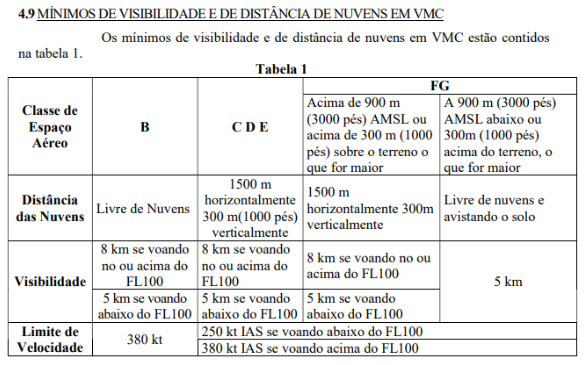
\includegraphics[width=0.9\linewidth]{figuras/vms.png}
        \label{fig:enter-label}
        \fonte{DACEA}
        }
    \end{figure}

\item Velocidade máxima de 120 km/h; 
    \item Altura de voo máxima de 120m; 
    \item Não requer comunicação bilateral com órgão ATS se estiver operando dentro dos limites estabelecidos; 
    \item Realizar operação VLOS, em área circular, polígono ou corredor, sendo limitada a uma distância horizontal que permita a manutenção da visualização da aeronave, com ou sem auxílio de um ou mais observadores; (Operação na qual o piloto, sem o auxílio de observadores de RPA, mantém o contato visual direto (sem auxílio de lentes ou outros equipamentos) com a aeronave remotamente pilotada, de modo a conduzir o voo com as responsabilidades de manter as separações previstas com outras aeronaves, bem como de evitar colisões com aeronaves e obstáculos”. Essa é a forma mais comum de se utilizar o drone, manter na linha de visada do piloto é uma forma que aumenta em muito a segurança).
    \item Afastamento mínimo de 30 m de pessoas não anuentes, animais e propriedades de terceiros com exceção dos órgãos de segurança pública;
    \item Afastamento mínimo de 9 km aeródromos cadastrados, quando operando nas zonas de aproximação e de decolagem;  
    \item Afastamento mínimo de 3 km do centro de helipontos cadastrados independente da altura do heliponto;
    \item Afastamento mínimo de 2 km de áreas nas quais sejam previstas operações ligadas à aviação agrícola.     
\end{enumerate}


\section{Liberação da empresa}

Para o funcionamento da empresa Drop Flash é necessário:\\

\textbf{Alvará de funcionamento (AFL)}
O Auto de Licença de Funcionamento (ALF) é o documento obrigatório que autoriza o funcionamento de atividades que não são residenciais, como comércios, indústrias ou serviços.\\

\textbf{Alvará de localização}
Para que a Drop Flash seja inaugurada no Brasil, é necessário verificar se o local onde o negócio será implantado está disponível. A inspeção técnica realizada pelo fiscal municipal é obrigatória.\\

\textbf{Licença prévia }
Durante o planejamento inicial, é possível solicitar uma Licença Prévia, para modificar ou expandir a estrutura de um estabelecimento. Este tipo de autorização garante que a empresa está em conformidade com os padrões ambientais necessários para a construção do negócio.\\

\textbf{Licença de instalação} 
A licença de instalação confirma que o projeto está em conformidade com as leis atuais e permite legalmente o início das obras no terreno.\\

\textbf{Licença de operação}
A obtenção de uma licença de operação é crucial para iniciar as operações do empreendimento. Quando emitida, indica que a empresa cumpriu os requisitos fundamentais e obrigatórios estabelecidos por lei para o planejamento, instalação e funcionamento do seu negócio.\\


% Funcionamento da plataforma drop flash
\chapter{Funcionamento da plataforma Drop Flash}
\label{ch:identificador}

\section{Cadastro para o Comerciante}

Para os comerciantes solicitarem entregas pela nossa plataforma é necessário realizar um cadastro diretamente pelo Site.

Ao entrar na plataforma o cliente será direcionado para realizar o login e senha se já for cadastrado já poderá realizar o login, caso não tenha o cadastro basta iniciar no ícone novo cadastro, após a realização do cadastro uma nova janela irá aparecer com vários ícones.

\begin{itemize}
    \item Acompanhar suas entregas;
    \item Solicitar uma nova entrega;
    \item Inserir novos credito para futuras entregas;
    \item Cancelar entrega;
    \item Alterar destino de entrega;
    \item Agendar entrega.
\end{itemize}

Conforme imagem abaixo da tela do Gestor onde o comerciante pode solicitar um novo pedido, acompanhar suas entregas, realizar novos créditos para futuras solicitações de entregas, verificar o saldo de créditos disponíveis, acesso ao suporte e monitorar em tempo real onde esta o entregador ou o drone.\\

\begin{figure} [!ht]
  { \centering
    \caption{Tela inicial do site}
    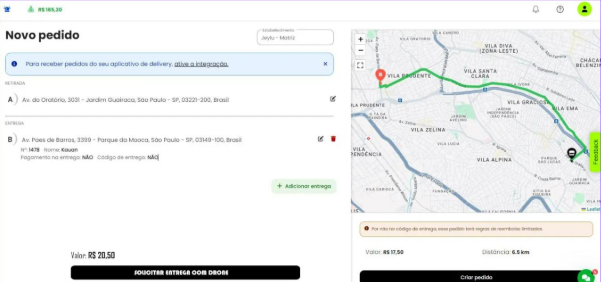
\includegraphics[width=0.5\linewidth]{figuras/funcionamento1.png}
    \label{fig:enter-label}
    \fonte{https://mottu.com.br}
    }
\end{figure}

Para solicitar um novo pedido basta clicar no ícone (novo pedido), o cliente será direcionado para o destino de retirada e local de entregas, pontos adicionais ou não, também será necessário colocar as especificações do produto a ser entregue ao cliente final, tamanho e peso do produto.

Com as informações de local de retirada e destino de entrega, dimensões e peso do produto, como por exemplo:\\

Solicitação de pedido:

\begin{itemize}
    \item Produto farmácia;
    \item Local de retirada e destino de entrega 2km ida e volta;
    \item Tamanho do pacote: 306 x 200 x 190 milímetros;
    \item Peso 1Kg.\\
\end{itemize}

Com essas informações a própria plataforma já vai informar os modelos ideais para esta entrega podendo o cliente optar por Moto ou drone.

\begin{itemize} 
    \item Opção Drone
    \begin{figure} [!ht]
       {\centering
        \caption{DFH - 1}
        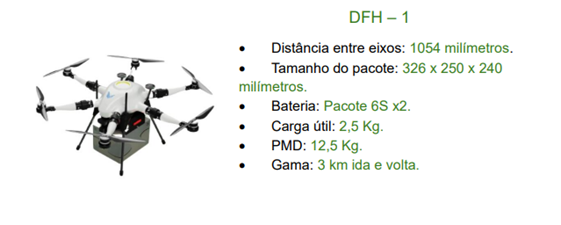
\includegraphics[width=0.9\linewidth]{figuras/drone dfh1.png}
        \label{fig:enter-label}
        \fonte{https://www.speedbird.aero}
        }
    \end{figure}
\\\\\\\\
    
    \item Opção Moto
    \end{itemize}

\begin{figure}[!ht]
    {
    \centering
    \caption{Drop - 110}
    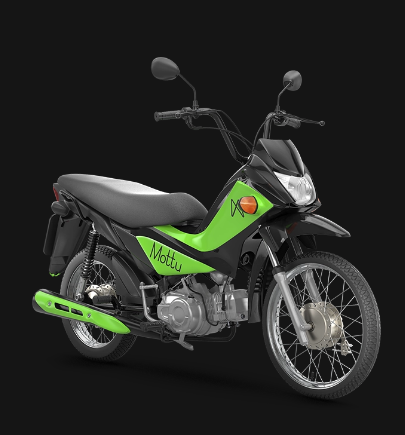
\includegraphics[width=0.5\linewidth]{figuras/Drop110.png}
    \label{fig:enter-label}
    \fonte{https://www.speedbird.aero}
    }
\end{figure}
    


Após finalizar a solicitação de entrega o pedido fica disponível para o entregador, no momento que o entregador aceitar a entrega o cliente poderá acompanhar o pedido em tempo real. O pedido disponível para o entregador, o cliente vai visualizar desta maneira para conseguir acompanhar a sua entrega com mais tranquilidade e transparência.

\begin{figure} [!ht]
   {\centering
    \caption{Acompanhamento do pedido pela plataforma}
    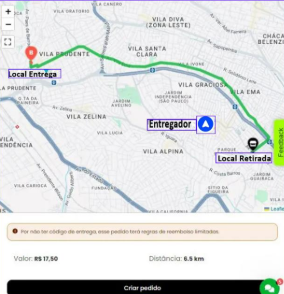
\includegraphics[width=0.4\linewidth]{figuras/pedido.png}
    \label{fig:enter-label}
    \fonte{https://mottu.com.br}
    }
\end{figure}

\section{Cadastro para o entregador}

Para os entregadores ter acesso as entregas pela nossa plataforma é necessários realizar um cadastro diretamente pelo Site ou pelo App disponível nas plataformas da Play Store e App Store. Ao entrar na plataforma o entregador será direcionado para realizar o login e senha se já for cadastrado já poderá realizar o login e realizar as entregas disponíveis, caso não tenha o cadastro basta iniciar no ícone novo cadastro, uma nova janela irá aparecer para o preenchimento do cadastro.

\begin{itemize}
    \item Dados pessoais;
    \item Foto da habilitação;
    \item Foto do rosto para realizar a comparação do documento informado;
    \item Documento do veículo.
\end{itemize}

Após o término do cadastro os dados serão analisados e se tudo 
estiver correto o entregador está apto a utilizar a plataforma. Com o cadastro aprovado o entregador realizará o login e senha, podendo escolher a entrega que estiver disponível na plataforma.\\

O Entregador vai visualizar os pedidos dessa maneira conforme imagem abaixo:

\begin{figure} [!ht]
   {\centering
    \caption{Tela inicial do App para entregadores}
    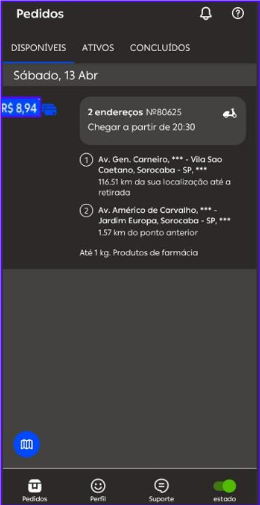
\includegraphics[height=0.5\linewidth]{figuras/app para entregadores.png}
    \label{fig:enter-label}
    \fonte{Borzo Courier}
    }
\end{figure}
\vspace{2cm}
 
Na tela inicial o entregador tem as informações do pedido:
\begin{itemize}
    \item Peso;
    \item Descrição do produto;
    \item Distância entre o entregador está para chegar ao ponto de retirada;
    \item Distância entre o ponto de retirada e entrega do produto.
    \item Valor da entrega;
    \item Hora de retirada e Hora de Entrega.
        \begin{figure} [!ht]
            {\centering
             \caption{Tela inicial do entregador com as informações do pedido}
             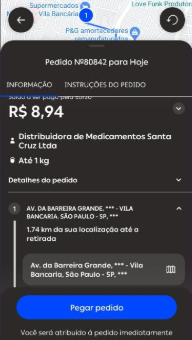
\includegraphics[width=0.5\linewidth]{figuras/infopedido.png}
             \label{fig:enter-label}
             \fonte{Borzo Courier}
            }
        \end{figure}

\end{itemize}

\begin{itemize}
Após o entregador aceitar a corrida na tela vai aparecer a seguinte mensagem:
Você tem certeza que é está rota que deseja?
\end{itemize}

\begin{figure} [!ht]
    {\centering
    \caption{Mensagem de confirmação de rota}
    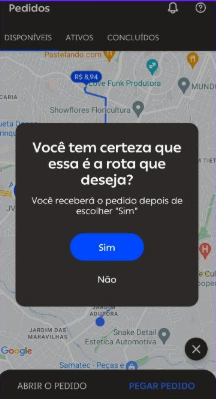
\includegraphics[height=0.5\linewidth]{figuras/mensagementregador.png} 
    \label{fig:enter-label}
    \fonte{Borzo Courier}
    }
\end{figure}

Caso o entregado não aceite a corrida ele é direcionado para a tela de pedidos disponíveis.\\

O entregador aceitando a entrega, ele será direcionado para a tela de rota do pedido e assim o entregador inicia a coleta do pedido para realizar a entrega.

\begin{figure} [!ht]
 {  \centering
    \caption{Tela da rota do pedido}
    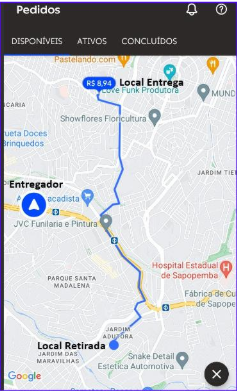
\includegraphics[width=0.3\linewidth]{figuras/rota do entregador.png}
    \label{fig:enter-label}
    \fonte{Borzo Courier}
    }
\end{figure}

Após o entregador finalizar a entrega uma avaliação de satisfação estará disponível para:

\begin{itemize}
    \item Estabelecimento
    \item Entregador
    \item Cliente final
\end{itemize}

A avalição chegará via app conforme imagem abaixo:

\begin{figure} [!ht]
   {\centering
    \caption{Tela de avaliação}
    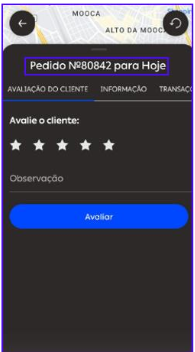
\includegraphics[width=0.5\linewidth]{figuras/avaliacao.png}
    \label{fig:enter-label}
    \fonte{Borzo Courier}
    }
\end{figure}

\begin{figure} [!ht]
   {\centering
    \caption{Tela avaliação finalizado}
    
\includegraphics[width=0.5\linewidth]{figuras/image.png}
    \label{fig:enter-label}
    \fonte{Borzo Courier}
    }
\end{figure}

Ao finalizar a entrega e a confirmação do produto solicitado pelo cliente final está tudo certo o valor referente a taxa de entrega já está disponível na conta do entregador que foi informado no momento do cadastro da plataforma.





%  Marketing das motos
\chapter{Marketing}
\label{ch:identificador}

\section{Aluguel de drone e motos}

\begin{figure} [!ht]
   { \centering
    \caption{DFH - 1}
    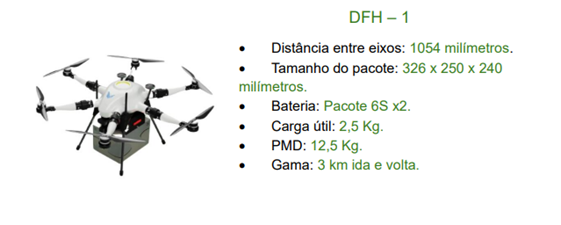
\includegraphics[width=0.6\linewidth]{figuras/drone dfh1.png}
    \label{fig:enter-label}
    \fonte{https://www.speedbird.aero/}
    }
\end{figure}

\begin{figure}[!ht]
   { \centering
    \caption{DFH - 2}
    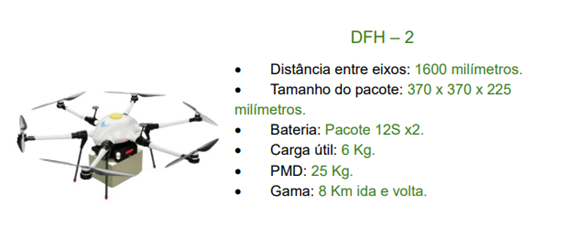
\includegraphics[width=0.6\linewidth]{figuras/drone dfh2.png}
    \label{fig:enter-label}
    \fonte{https://www.speedbird.aero/}
    }
\end{figure}

\begin{figure}[!ht]
   { \centering
    \caption{DFH - 4}
    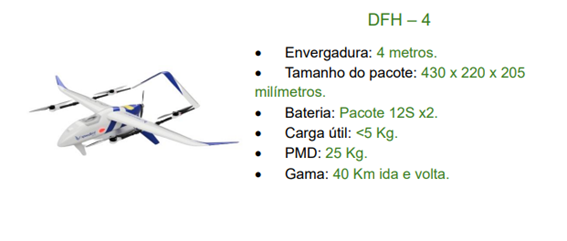
\includegraphics[width=0.6\linewidth]{figuras/drone dfh4.png}
    \label{fig:enter-label}
    \fonte{https://www.speedbird.aero/}
    }
\end{figure}

\section{Motos}

\begin{figure} [!ht]
  { \centering
    \caption{Nossas Motos}
    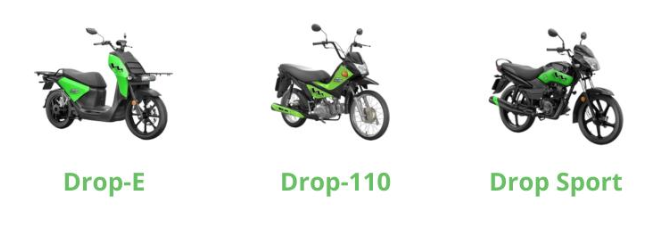
\includegraphics[width=0.75\linewidth]{figuras/motos.png}
    \label{fig:enter-label}
    \fonte{https://mottu.com.br/aluguel/}
    }
\end{figure}

Todos nossos planos contratados incluem:

\begin{figure} [!ht]
   { \centering
    \caption{Benefícios dos planos de contrato}
    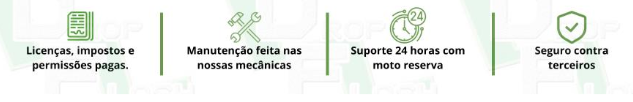
\includegraphics[width=0.9\linewidth]{figuras/PLANO.png}
    \label{fig:enter-label}
    \fonte{https://mottu.com.br}
    }
\end{figure}

Entregadores disponíveis por São Paulo:

\begin{figure} [!ht]
   { \centering
    \caption{Entregadores 24 horas em diversos pontos de São Paulo}
    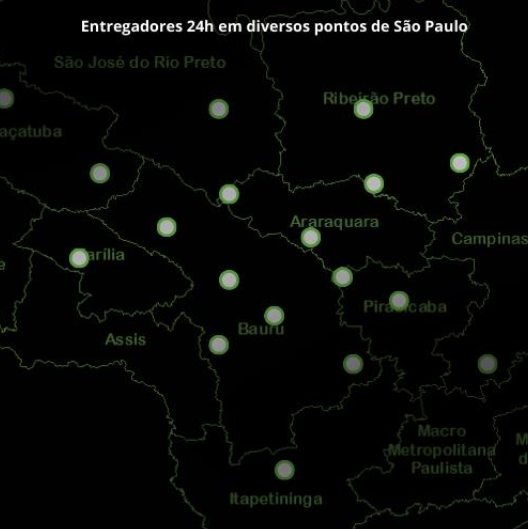
\includegraphics[width=0.4\linewidth]{figuras/ENTREGADOREMSP.png}
    \label{fig:enter-label}
    \fonte{https://mottu.com.br}
    }
\end{figure}

\section{Parcerias}

\begin{figure} [!ht]
   { \centering
    \caption{Principais Parceiros}
    
\includegraphics[width=0.9\linewidth]{figuras/principaisparceiros.png}
    \label{fig:enter-label}
    \fonte{Drop Flash (criado por nós)}
    }
 \end{figure}   

 \section{Integrações}

 \begin{figure} [!ht]
   { \centering
    \caption{Integrações}
    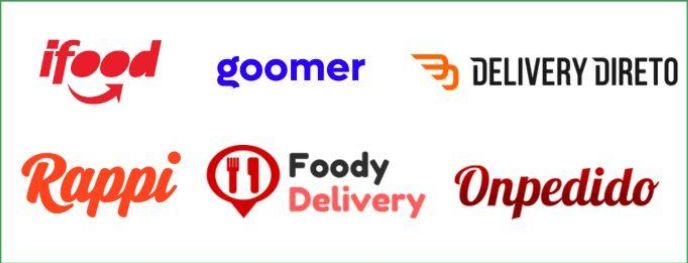
\includegraphics[width=0.9\linewidth]{figuras/integracoes.png}
    \label{fig:enter-label}
    \fonte{Drop Flash (criado por nós)}
    }
\end{figure}  

\vspace{3.0cm}

\section{Proposta financeira}

\begin{figure}[!ht]
    {\centering
    \caption{Proposta Financeira}
    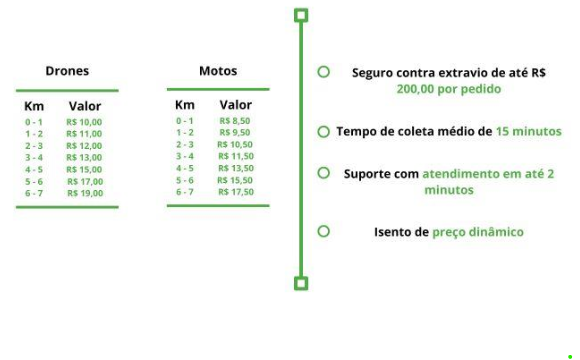
\includegraphics[width=0.5\linewidth]{figuras/financeiro.png}
    \label{fig:enter-label}
    \fonte{Drop Flash (criado por nós)}
    }
\end{figure}


\section{Contato}

\begin{figure} [!ht]
   { \centering
    \caption{Contato}
    
\includegraphics[width=0.7\linewidth]{figuras/contato.png}
    \label{fig:enter-label}
    \fonte{Drop Flash (criado por nós)}
    }
 \end{figure}   





% Robo
\chapter{Robô}
\label{ch:identificador}

\section{Apresentação Steve Robot Express}

Nós da Drop Flash realizamos além das entregas já mencionadas o serviço de entregas voltada para condomínios comerciais, residências e Shoppings centers chamado Steve Robot Express. Com a Steve Robot Express disponibilizamos aluguéis de robôs de quatro rodas que se movem livremente realizando a entregas    de comida documentos e pequenos pacotes até trinta quilos atendendo as necessidades dos nossos clientes. Usado em um condomínio por exemplo o robô Steve poderia realizar a emprega de pedidos sem a necessidade de o morador descer até a portaria pois o Steve faria isso para você trazendo o pedido até sua porta trazendo mais conforto e praticidade otimizando o tempo de todos, o morador teria apenas que solicitar o serviço por meio de um aplicativo de smartphone e utilizar o mesmo para desbloquear e abrir o compartimento de carga e retirar o seu pedido \cite{BoysenN2018}.

Para implantação do Steve em um condomínio levaremos em conta a quantidade de residências, pedidos recebidos em um mês, distância percorrida e tempo máximo de entrega para a unidade mais longe. Com esses dados conseguimos mensurar a quantidade de robôs a serem instalados.

Em uma implantação que realizamos em um condomínio de 328 unidades com 1.387 pedidos recebidos na portaria por mês chegamos na média de 4,2 pedidos por unidade, calculando que o tempo máximo de entrega para a moradia mais longe seria de 10 minutos, com todos esses dados realizamos o cálculo do tempo mensal de entregas = 328 x 4,2 x 10 chegamos no resultado de 13.776 minutos. Nosso robô Steve tem autonomia de 12 horas mas para garantir uma maior durabilidade eles trabalham apenas 8 horas por dia o que seria equivalente a 480 minutos por dia ou 14.400 minutos por mês sabendo disso realizamos o ultimo cálculo para saber quantos robôs são necessários para atender o condômino 13.776 / 14.400 chegamos ao resultado de 0,95 a arredondando chegamos à conclusão de que seira necessário um robô para realizar as entregas em todas as 328 unidades do condomínio mas por motivos de segurança e picos de pedidos recebidos em horas especificas orientamos a instalação de duas unidades do Steve para uma entrega mais rápida e dinâmica.

O Steve também conta com diversas funcionalidades projetado para otimizar o processo de entregas funciona de forma autônoma com uma tecnologia que conta com mais de dez câmeras garantindo uma visão de trezentos e sessenta graus, sensores ultrassônicos, navegação GPS, permitindo que a inteligência artificial detecte obstáculos e tome decisões, como desviar ou parar até que um obstáculo móvel passe. Nosso Robô Steve também consegue diferenciar calçadas, ruas, grama, ciclovia e árvores, mesmo em ambientes externos. Steve também conta com sistemas de comunicação (IoT) Internet das coisas e (M2M) Machine-to-Machine sendo o M2M fundamental na IoT, permitindo que dispositivos troquem informações diretamente entre si, sem intervenção humana montando uma memória colaborativa de rotas, com o objetivo de criar uma navegação autônoma cada vez mais precisa criando um mapa com características especificas dos ambientes tornando as viagens cada vez mais rápidas, Além de garantir uma interação maior com outros equipamentos eletrônicos no caso do Steve seria a comunicação com sistemas de elevadores permitindo sua movimentação sem problemas em todos os andares do edifício. Garantindo assim total autonomia do Steve a implantação do sistema IoT nos elevadores e feita em conjunto com a Dusun IoT \cite{DusunIot} especializada em hardware e gateways IoT fornecendo todos os dispositivos necessários. Já os pontos de recarga são instalados em conjunto com a Synkar, companhia brasileira especializada em inteligência artificial que disponibiliza toda a parte de software, automação, manutenção e reposição de peças sendo ela a responsável por fabricar e disponibilizar todos os robôs Steve. Visando também na diminuição dos impactos ambientais todos os robôs produzidos são 100\% elétricos os tornando ecologicamente corretos, contribuindo para a redução das emissões de gases do efeito estufa (GEE) e também do congestionamento em grandes cidades \cite{Bakach2020}

\section{Especificações do Steve} 
\begin{figure} [!ht]
   { \centering
    \caption{Ilustração robô de entregas da empresa Synkar}
    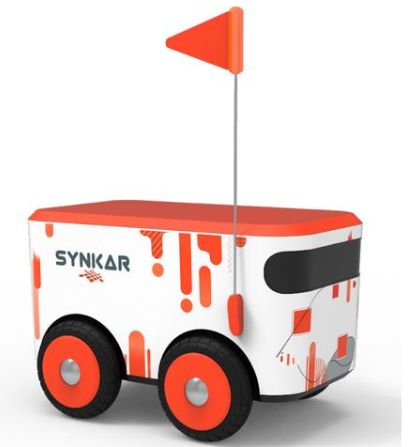
\includegraphics[width=0.5\linewidth]{figuras/synkar.png}
    \label{fig:enter-label}
    \fonte{https://www.synkar.com/ourrobots/}
    }
\end{figure}

Capacidade de transporte: 30 kg Veículo: 100\% elétrico
Autonomia: 12 horas Navegação: Autônoma por Inteligência Artificial
Sistema: Machine-to-Machine Atuação na primeira e Última milha
API: Drop Flash Steve API (DFSA) Fabricante: Synkar

\section{Logística Interna e Externa}
Compreendemos que as operações do mundo real não se restringem a um único cenário. Portanto, nossos robôs têm a capacidade de operar tanto em ambientes internos quanto externos.

\begin{figure} [!ht]
    {\centering
    \caption{Diferentes formas de interpretação dos ambientes através de câmeras}
    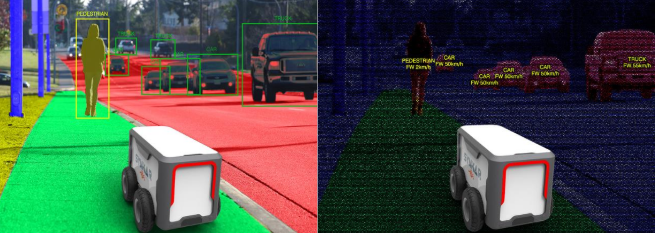
\includegraphics[width=0.5\linewidth]{figuras/stevelogistica.png}
    \label{fig:enter-label}
    \fonte{https://www.synkar.com/ourrobots/}
    }
\end{figure}

\section{Navegação Por Inteligência artificial}
Acreditamos que a automação está moldando o futuro. Nossos robôs têm a capacidade de proporcionar segurança, rapidez e consistência nas operações dos nossos parceiros.

\begin{figure}[!ht]
   { \centering
    \caption{Demonstração da capacidade de tomada de decisão ao encontrar obstáculos}
    \includegraphics[width=0.5\linewidth]{figuras/stevenavegaçao.png}
    \label{fig:enter-label}
    \fonte{https://www.synkar.com/ourrobots/}
    }
\end{figure}

\section{API customizável para os parceiros}
A Drop Flash Steve API (DFSA) é altamente flexível e pode ser adaptada às necessidades específicas dos nossos parceiros. Ela oferece desde operações logísticas básicas até a possibilidade de desenvolver funcionalidades personalizadas.

\section{Curiosidades}
Escolhemos o nome de Steve para o nosso robô em homenagem a Steve Jobs que com seus feitos revolucionou a área da tecnologia deixando seu legado e servindo de exemplo para as novas gerações por sua criatividade e visão que moldaram a forma com interagimos com a
tecnologia até hoje. Nós da Drop Flash seguimos o mesmo caminho revolucionando na área de entregas buscando a cada dia trazer mais economia de tempo e praticidade aos nossos clientes com novas tecnologias sustentáveis.

% Financeiro
\chapter{Orçamento do Steve}
\label{ch:identificador}

\section{Custos de implementação}
Inicialmente realizaremos a implementação do Steve Robot Express nas principais capitais e regiões metropolitanas das regiões Sul, Sudeste e Centro Oeste totalizando onze capitais para comercialização, realizando em média dez implementações mensais em cada uma das capitais totalizando 110 implementações ao mês 1.320 por ano.

\section{Custo do robô Steve}
Nossos robôs Steve são produzidos em parceria com a empresa Synkar,
companhia brasileira especializada em inteligência artificial que disponibiliza toda a parte de software, automação, manutenção e reposição de peças. O valor de produção robô Steve e entorno de US\$ 5.000 em reais R\$ 26.036,00 com base no valor dos robôs da empresa Starship Technologies.

\section{Custo médio do ponto de recarga}
O valor gasto na adequação dos condomínios ficaria algo entre US\$ 288,06 a US\$ 960,21 dólares em reais algo entre R\$1.500,00 a R\$5.000.00 totalizando um custo médio de US\$ 624,14 dólares R\$ 3.250,00 reais. Pois para a implementação dos pontos de recarga são necessários um projeto elétrico que contenha desenho da rede elétrica cálculos de dimensões e especificações dos equipamentos utilizados também e necessário a ART (Anotação de Responsabilidade Técnica) que é um documento padrão de engenharia registrado junto ao CREA da documentação técnica do projeto. Os valores acima foram baseados em carregadores de automóveis elétricos de um artigo do site CondoCash \cite{CondoCash}.

\section{Instalação hardware e software IoT para elevador}
Para instalação dos sistemas de hardware e software realizamos uma parceria com uma grande empresa chinesa Dusun IoT \cite{DusunIot} especializada em hardware gateways IoT permitindo a comunicação do Steve com o elevador além dessa comunicação permitirá que o condomínio tenha em mãos dados de monitoramento em tempo real e desempenho do elevador, possibilitando a manutenção preditiva prevendo falhas antes que ocorram e otimização do consumo de energia do elevador com base em dados pesquisados os custos de hardware com sensores, módulos Wi-Fi, Bluetooth, Placas como o Raspberry Pi, Arduino, câmeras de segurança IoT, rastreadores GPS, placas, cabos e documentação variando de R\$ 1.500,00 a R\$ 1.800,00 reais, com um custo médio de R\$ 1.650,00 reais. Os valores das peças foram retirados dos principais Marketplaces do Brasil. Já o software ficara em torno de US\$ 10.000,00 dólares algo entre R\$52.072 reais em valores aproximados de acordo com o site ICHI.PRO \cite{ICHI.PRO} mas uma vez desenvolvido o software poderia ser usado utilizado em todas as instalações havendo apenas pequenas atualizações. 

\section{Custos operacionais mensais nas onze capitais}
Os custos operacionais relacionados a reposição de peças em estoque totalizam R\$ 2.000,00 reais por capital totalizando um custo mensal nas onze capitais de R\$ 22.000,00, além do custo das peças temos os custos com técnico de mecatrônica que é de R\$ 5.200,00 reais por capital totalizando um custo mensal com técnicos de R\$ 57.200,00 reais nas onze capitais. Totalizando R\$ 79.400,00 de custos operacionais mensais.

\section{Custos totais para viabilização da Steve Robot Express}
Com um investimento inicial de R\$ 90.208,00 para a viabilização da Steve Robot Express, na primeira capital, mas vendo abaixo um modelo de implementação ficara mais claro ver que o retorno do investimento e muito atrativo e escalável trazendo retornos consideráveis em alguns anos.

\textbf{Exemplo de implantação}
Dados de implementação do Steve Robot Express em um condomínio com 328 residentes que necessitaria de dois Steve Robots para realização de todas as entregas.

\textbf{Dados usados para a base de cálculo:}
\begin{itemize}
    \item Custo Steve Robot 2 unidades: R\$ 52.072,00
    \item Custo Bases de recarga 1 unidade: R\$ 3.250,00
    \item Custo médio Elevador Smart hardware 2 unidades: R\$ 3.300,00
    \item custos operacionais mensais: R\$ 7.200,00
    \item custo total para implementação: R\$ 65.822,00
    \item Valor recebido do condomínio para implementação: R\$ 100.000,00
    \item Parcelas mensais recebidas do condomínio para 2 unidades do Steve Robot: R\$ 8.250,00
\end{itemize}

\textbf{Cálculo implantação:}
Para calcular o lucro retorno sobre o investimento em um período de doze meses, realizaremos a subtração dos custos totais do valor recebido durante o período de doze meses.

Custo Total= R\$ 65.822,00 + R\$ 86.400,00 = R\$ 152.222,00 reais, o custo total e a soma da implantação mais os custos operacionais durante os doze meses.

Agora calcularemos o valor recebido da implantação mais os pagamentos mensais.

Valor Total Recebido = R\$ 100.000,00 + R\$ 99.000,00 = R\$ 199.000,00 reais

Agora para calcular o retorno sobre o investimento, vamos subtrair o custo total do valor total recebido.

Lucro / Retorno = R\$ 199.000,00 – R\$ 152.222,00 = R\$ 46.778,00 reais

Após os cálculos concluímos que o retorno sobre o investimento para a implementação do Steve Robot Express retornaria ao final de doze meses 30,75\% totalizando um lucro de R\$ 46.778,00 da implementação em apenas um condomínio. 

\section{Retorno dos investimentos da Steve Robot Express}
Com o lucro de apenas uma implementação retornando R\$ 46.778,00 reais se multiplicarmos esse valor por 110 implementações mensais teríamos o valor de R\$ 5.145.580,00 reais que em um ano seria o equivalente a R\$ 61.746.960,00.

Estudo da consultoria Boston Consulting Group (BCG) \cite{(BCG)} prevê que robôs de serviço deverão se tornar líderes no setor da robótica até o final da década o que representaria US\$ 90 bilhões a US\$ 170 bilhões do faturamento global em 2030 para a categoria. O estudo abrange diversas mudanças elas estão relacionadas ao envelhecimento da população que necessitarão de ajuda na realização de tarefas, mudanças no comportamento da população aumentando a demanda de entregas de produtos cada vez mais rápida e personalizada sem falar da conscientização da população em relação a ações mais sustentáveis que levarão a modernização e maior uso dos robôs.

Outra previsão realizada prevê que o tamanho mercado de robótica é estimado em US\$ 45,85 bilhões em 2024, e deverá atingir US\$ 95,93 bilhões até 2029, crescendo a um CAGR de 15,91\% durante o período de previsão (2024-2029). Foi observado numerosos investimentos no setor por conta da revolução da Industria 4.0 que são um dos elementos chave para o desenvolvimento dos robôs o gráfico abaixo mostra uma projeção do desenvolvimento e crescimento do mercado até onfim dessa década. 

\begin{figure} [!ht]
    \centering
    \caption{Indústria de robótica - Análise de tamanho e participação - Tendências e previsões de crescimento (2024 - 2029)}
    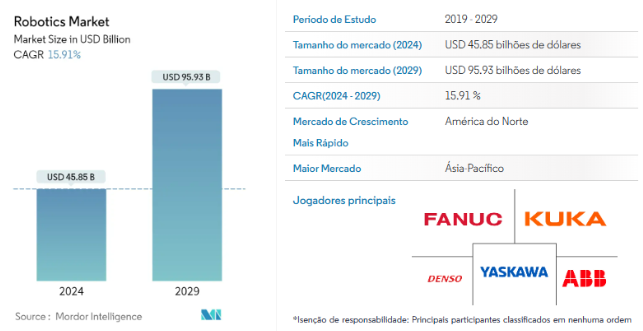
\includegraphics[width=0.9\linewidth]{figuras/orça drop.png}
    \label{fig:enter-label}
    \fonte{Mordor Intelligence Research & Advisory}
\end{figure}

Com as previsões dessas instituições fica claro que o cenário da robótica só está no começo como uma empresa pioneira a Drop Flash vem com missão de a cada dia aproximar o cidadão comum com tecnologias que em alguns anos se tornarão essenciais para garantir a qualidade nas entregas. 

% Marketing da empresa 
\chapter{Marketing do Steve Robot Express}
\label{ch:identificador}

\begin{figure} [!ht]
    \centering
    \caption{Sobre nosso serviço}
    \includegraphics[width=1.0\linewidth]{figuras/mark1.jpeg}
    \fonte{Drop Flash (criado por nós)}
    \label{fig:enter-label}
\end{figure}

\begin{figure} [!ht]
    \centering
    \caption{Serviços disponíveis nas Regiões}
    \includegraphics[width=1.0\linewidth]{figuras/mark2.jpeg}
    \fonte{Drop Flash (criado por nós)}
    \label{fig:enter-label}
\end{figure}

\begin{figure} [!ht]
    \centering
    \caption{Nosso diferencial}
    \includegraphics[width=1.0\linewidth]{figuras/mark3.jpeg}
    \fonte{Drop Flash (criado por nós)}
    \label{fig:enter-label}
\end{figure}

\begin{figure} [!ht]
    \centering
    \caption{Principais parceiros}
    \includegraphics[width=1.0\linewidth]{figuras/mark4.jpeg}
    \fonte{Drop Flash (criado por nós)}
    \label{fig:enter-label}
\end{figure}

\begin{figure} [!ht]
    \centering
    \caption{Integrações}
    \includegraphics[width=1.0\linewidth]{figuras/mark5.jpeg}
    \fonte{Drop Flash (criado por nós)}
    \label{fig:enter-label}
\end{figure}

\begin{figure} [!ht]
    \centering
    \caption{Proposta Financeira}
    \includegraphics[width=1.0\linewidth]{figuras/mark6.jpeg}
    \fonte{Drop Flash (criado por nós)}
    \label{fig:enter-label}
\end{figure}

\begin{figure} [!ht]
    \centering
    \caption{Drop Flash}
    \includegraphics[width=1.0\linewidth]{figuras/mark7.jpeg}
    \fonte{Drop Flash (criado por nós)}
    \label{fig:enter-label}
\end{figure}

% Proposta de contrato
\chapter{Proposta de venda}
\label{ch:identificador}

\section{Proposta Financeira}
Nossa proposta financeira dispõe de implantação do sistema com 50\% pagos na assinatura do contrato os outros 50\% podem ser parcelados em 60x com correção de juros anuais junto às parcelas mensais.

Usando o Condomínio com 328 residentes como exemplo podemos ver que os custos para implantação ficariam dentro do orçamento de todos os moradores:

O custo inicial para implantação é de R\$ 100.000,00 reais desse valor damos a opção do condomínio realizar o parcelamento de 50\% desse valor o que levaria a um custo inicial para implantação de R\$ 50.000,00 reais divididos para os 328 moradores chegaríamos ao valor de R\$ 152, 43 por morador. Já os outros 50 mil parcelados poderiam ser parcelados em ate 60 meses com uma taxa de juros pre estabelecida variando de acordo com a escolha do condomínio.

\section{Opções de parcelamento implantação mais parcelas mensais}

\textbf{Parcelamento em 12 meses:}
Pagamento dos 50\% em 12 meses com taxa de juros a 4\% ficaria doze parcelas de R\$ 6.166,66 mais parcelas mensais de R\$ 8.250,00 chegando a parcelas mensais de R\$ 14.466,66 esse valor dividido entre os 328 moradores do condomínio ficaria R\$ 43,95 por mês após a quitação dos 50\% parcelados o valor da parcela cairia para R\$ 25,15 para cada morador do condomínio.

Para parcelamentos acima de 12 meses e cobrado, um acréscimo de 0,5% ao ano

\textbf{Parcelamento em 24 meses:}
Pagamento dos 50\% em 24 meses com taxa de juros a 4,5\% ficaria doze parcelas de R\$ 4.208,33 mais parcelas mensais de R\$ 8.250,00 chegando a parcelas mensais de R\$ 12.458,00 esse valor dividido entre os 328 moradores do condomínio ficaria R\$ 37,98 por mês após a quitação dos 50\% parcelados o valor da parcela cairia para R\$ 25,15 para cada morador do condomínio.

\textbf{Parcelamento em 36 meses:}
Pagamento dos 50\% em 36 meses com taxa de juros a 5\% ficaria doze parcelas de R\$ 3.638,88 mais parcelas mensais de R\$ 8.250,00 chegando a parcelas mensais de R\$ 11.888,88 esse valor dividido entre os 328 moradores do condomínio ficaria R\$ 36,24 por mês após a quitação dos 50\% parcelados o valor da parcela cairia para R\$ 25,15 para cada morador do condomínio.

\textbf{Parcelamento em 48 meses:}
Pagamento dos 50\% em 48 meses com taxa de juros a 5,5\% ficaria doze parcelas de R\$ 3.3416,66 mais parcelas mensais de R\$ 8.250,00 chegando a parcelas mensais de R\$ 11.666,66 esse valor dividido entre os 328 moradores do condomínio ficaria R\$ 35,56 por mês após a quitação dos 50\% parcelados o valor da parcela cairia para R\$ 25,15 para cada morador do condomínio.

\textbf{Parcelamento em 60 meses:}
Pagamento dos 50\% em 60 meses com taxa de juros a 6\% ficaria doze parcelas de R\$ 3.333,33 mais parcelas mensais de R\$ 8.250,00 chegando a parcelas mensais de R\$ 11.583,33 esse valor dividido entre os 328 moradores do condomínio ficaria R\$ 35,31 por mês após a quitação dos 50\% parcelados o valor da parcela cairia para R\$ 25,15 para cada morador do condomínio.



%Regulamentação 
\chapter{Regulamentação de robôs entregadores}
\label{ch:identificador}

No brasil as regulamentações dos robôs entregadores ainda estão em 
desenvolvimento, mas já existem algumas diretrizes gerais que podem ser  aplicadas com base nas regras existentes como a NR 12 Norma Reguladora \cite{NR12} criada em 1978 (lei 3.214), criada pelo governo federal com o objetivo de estabelecer os parâmetros técnicos e quais regras cumprir para oferecer proteção no trabalho com diferentes maquinários. Dentro dessa área temos também a ISO/TS 15066 \cite{ISO/TS15066} voltada para robôs colaborativos sendo um complemento da ISO 10218 \cite{(ISO10218)} que fala sobre “Requerimentos de Segurança para Robôs Industriais”.

Com base nessas normas podemos encontrar regras já existentes para dispositivos autônomos e veículos que devem ser considerados na implantação do nosso robô de entregas Steve sendo essas.

\textbf{Segurança:} Garantir que os robôs sejam projetados com dispositivos de segurança evitando acidentes com pedestres e automóveis. Permitindo que sejam capazes de evitar obstáculos e interagir de forma segura com o ambiente.

\textbf{Tráfego:} Implementação de regras especificas para circulação dos robôs nas vias de condomínios residenciais, como limites de velocidade, uso de faixas e sinalização adequada.

\textbf{Privacidade:} Garantir a proteção de dados e a privacidade dos cidadãos, o que inclui a gestão das informações coletadas pelos sensores dos robôs durante a entrega.

\textbf{Responsabilidade:} A Drop Flash junto a Synkar nos responsabilizamos por danos ou acidentes envolvendo robôs entregadores caso ocorram prestando auxílio em possíveis ocorrências. 

\textbf{Homologação:} Com base na NR 12 e ISO/TS 15066 buscamos junto aos órgãos competentes garantir que atendam aos padrões técnicos e de segurança exigidos.

\textbf{Operação Comercial:} Para obtenção de permissões para operações comerciais em diversas capitais entramos em contato com órgãos reguladores para obtenção de licenças ou autorizações dependendo das regras de cada estado

Nos Estados Unidos a Federal Aviation Administration \cite{faa2018} estabelecem menos regulamentações de segurança em áreas de pilotagem de aeronaves para robôs autônomos facilitando assim a implantação dos robôs em aeroportos ou locais próximos a áreas de carga e descarga de aeronaves. 

% Conclusão
\chapter{Conclusões}
\label{ch:conclusao}

A operação da Drop Flash, uma empresa de entregas que utiliza tecnologias avançadas, incluindo robôs autônomos, como o Steve Robot Express, e drones de diferentes capacidades. Inicialmente, detalhou-se a operacionalização da Drop Flash conectando clientes a entregadores independentes e estabelecendo um sistema de taxas baseado na distância percorrida e na demanda regional. Especificamente, a implementação do Steve Robot Express em condomínios foi minuciosamente analisada, considerando fatores como o número de residências, pedidos mensais, distância percorrida e tempo de entrega. Calculou-se a necessidade de robôs com base na autonomia e capacidade operacional dos Steve Robots, sugerindo a instalação de duas unidades para assegurar eficiência e rapidez nas entregas. As características técnicas dos Steve Robots, incluindo suas múltiplas câmeras, sensores ultrassônicos e sistemas de navegação GPS, foram destacadas como fundamentais para a operação segura e eficiente em ambientes diversos. Além disso, o documento explorou os custos e o retorno sobre o investimento para a implementação dos Steve Robots. A análise financeira indicou um retorno atrativo de 30,75\% ao final de doze meses para um condomínio de 328 unidades, demonstrando a viabilidade econômica do projeto. A Drop Flash também investe em drones para otimizar entregas rápidas e de menor peso. Os drones DLV-1 e DLV-2 foram descritos com suas respectivas capacidades de carga e distâncias operacionais, destacando suas vantagens para entregas urgentes e de maior peso, respectivamente. Por fim, discutiu-se as vantagens do tráfego pago para a empresa, ressaltando a capacidade de gerar resultados imediatos, focar nas conversões e a flexibilidade de orçamento. O tráfego pago permite uma segmentação avançada e uma estratégia baseada em dados, essencial para o aprimoramento contínuo das campanhas publicitárias e maximização dos resultados. Conclui-se que a Drop Flash, ao integrar robôs autônomos e drones em suas operações, não apenas melhora a eficiência e rapidez das entregas, mas também se posiciona de forma competitiva no mercado emergente de robótica de serviços. A análise detalhada dos custos, retorno sobre o investimento e as estratégias de marketing reforçam a sustentabilidade e escalabilidade do negócio, prometendo um crescimento significativo nos próximos anos.

% ##################### Fim dos Capítulos ############################

% Bibliografia 
\bibliography{refs}

\end{document}